\documentclass[preprint,12pt,authoryear]{elsarticle}

\usepackage{amssymb,amsmath}
\usepackage{booktabs}
\usepackage[pageanchor=false]{hyperref}
\usepackage{graphicx}
\usepackage{xcolor}
\usepackage{multirow}
\usepackage{array}
\usepackage{microtype}
\usepackage{lineno}
\linenumbers
\setlength{\emergencystretch}{3em}
\hbadness=10000
\setlength{\hfuzz}{200pt}

\journal{Knowledge-Based Systems}

\begin{document}

\begin{frontmatter}

\title{Beyond Accuracy: A Validation Framework for Machine Learning in Cryptocurrency Trading}

\author{Jaewook Kim}
\address{Independent Researcher, Uijeongbu, Republic of Korea; B.S.\ Industrial Engineering, UNIST; Professional Engineer (Engineers Australia)}

\begin{highlights}
\item First financial ML validation checklist: 12-item VALID framework proposed
\item Bull bias: tree-based crypto ML models predict 90--97\% long without class balancing
\item Statistical signals (PBO$=$0, $p$=0) do not guarantee economic profitability
\item Transaction costs consume 55--91\% of ML alpha across four timeframes
\item Monte Carlo ($n$=200): 27\% AUC false positive rate; first Witzany (2021) PBO test
\end{highlights}

\begin{abstract}
Machine learning strategies for cryptocurrency trading routinely report exceptional backtest results, yet practitioners consistently fail to replicate them. We identify three systematic failure modes---directional prediction bias, statistical-economic disconnect, and transaction cost omission---through 340 strategy variants across four timeframes and three cryptocurrency assets. To address these failures, we propose VALID (Validation Architecture for Learning-based Investment Decisions), a 12-item reporting and validation framework for financial ML research---the first domain-specific checklist for this field.

We demonstrate that gradient-boosted models predict long 90--97\% of the time without class balancing; that standard validation tools (PBO\,=\,0, permutation $p$\,=\,0) cannot distinguish exploitable signals from noise; and that transaction costs consume 55--91\% of gross alpha. Monte Carlo analysis (200 iterations $\times$ 4 asset-timeframe settings) shows 27--30\% false positive rates for AUC-based validation alone, reduced to 0\% by CPCV with PBO. We provide the first empirical confirmation of \citeauthor{witzany2021bayesian}'s (\citeyear{witzany2021bayesian}) PBO critique through null-distribution analysis. A systematic audit of 80 papers reveals that the median study satisfies only 2.5 of 12 VALID items. We release an open-source implementation for reproducibility.
\end{abstract}

\begin{keyword}
financial machine learning \sep cryptocurrency trading \sep validation framework \sep backtest overfitting \sep reporting standard
\JEL G11 \sep G14 \sep G17 \sep C45 \sep C52
\end{keyword}

\end{frontmatter}

%% ================================================================
\section{Introduction}
\label{sec:intro}

The application of machine learning to cryptocurrency trading has grown rapidly, producing a literature characterized by strikingly positive results. Cross-sectional factor models report weekly long-short returns of 3.87\% \citep{fieberg2025ctrend}. LSTM ensembles achieve annualized Sharpe ratios exceeding 3.0 \citep{xu2022machine}. Tree-based models demonstrate AUC scores above 0.80 on directional prediction tasks \citep{li2024cryptocurrency}. Taken at face value, these findings suggest ML-driven crypto trading offers among the highest risk-adjusted returns in any asset class.

Yet the gap between published results and practitioner experience is vast. In traditional finance, this disconnect is well documented: \citet{ioannidis2005false} demonstrated that most published research findings are false under conditions of low pre-study odds and high researcher flexibility. \citet{harvey2016cross} showed that the majority of 316 published equity factors are likely false discoveries, proposing a $t$-ratio threshold of 3.0 rather than the conventional 2.0. \citet{mclean2016academic} documented 26\% out-of-sample decay and 58\% post-publication decay in equity anomalies. \citet{hou2020replicating} replicated 452 anomalies and found 65\% fail---82\% after multiple testing correction. The cryptocurrency ML literature has not yet undergone equivalent scrutiny.

\citet{kapoor2023leakage} identified data leakage affecting 294 studies across 17 scientific fields, proposing a taxonomy of eight leakage types and a ``model info sheet'' reporting template. Their work, published in \textit{Patterns} and subsequently extended to the REFORMS framework in \textit{Science Advances} \citep{kapoor2024reforms}, demonstrated that domain-specific validation standards can substantially reduce false positive rates. However, no analogous standard exists for financial ML. TRIPOD+AI \citep{collins2024tripodai} covers clinical prediction models. REFORMS addresses general ML-based science. MI-CLAIM \citep{norgeot2020mi} targets clinical AI. Not one published checklist addresses the unique challenges of ML-based trading strategy development: temporal data dependencies, transaction cost modeling, class imbalance in directional prediction, or the distinction between statistical and economic significance.

This gap has consequences. Without standardized validation, published crypto ML results vary wildly in methodological rigor. Some studies omit transaction costs entirely; others use unrealistically low cost assumptions. Few test for directional prediction bias. Even fewer apply advanced overfitting diagnostics such as Combinatorial Purged Cross-Validation (CPCV) or Probability of Backtest Overfitting (PBO), despite their demonstrated superiority over traditional walk-forward methods \citep{arian2024backtest}.

\subsection{Contributions}

This paper makes five contributions:

\begin{enumerate}
\item \textbf{The VALID framework.} We propose a 12-item validation and reporting checklist for financial ML research---the first domain-specific standard for this field.

\item \textbf{Systematic literature audit.} We survey 80 published cryptocurrency ML trading papers (2018--2026), coding each for validation methodology, cost assumptions, class balancing, baseline comparison, and code availability.

\item \textbf{Three empirical failure modes at scale.} Using 340 strategy variants across four timeframes and three cryptocurrency assets (BTC, ETH, SOL), we document: (a) bull bias, (b) statistical-economic disconnect, and (c) cost illusion.

\item \textbf{Monte Carlo false positive quantification.} We generate 200 synthetic price series per setting across four asset-timeframe configurations, demonstrating that AUC-based evaluation produces 27--30\% false positives while CPCV\,+\,PBO reduces this to 0\% [0\%, 1.9\%] in every setting. Ablation analysis identifies CPCV/PBO (Item V4) as the single most impactful validation component.

\item \textbf{Empirical validation of Witzany's PBO critique.} Through 200-iteration Monte Carlo simulation, we derive the first null distribution of $\mathrm{Var}(\mathrm{SR}_{\mathrm{IS}})$, demonstrating that PBO\,=\,0.000 reflects parameter-space flatness (real Var\,=\,0.012) rather than signal robustness (null 95th percentile\,=\,0.328).
\end{enumerate}

\subsection{Notation and Abbreviations}

Table~\ref{tab:glossary} defines the key terms used throughout this paper.

\begin{table}[htbp]
\centering
\caption{Key abbreviations and definitions.}
\label{tab:glossary}
\small
\begin{tabular}{lp{10cm}}
\toprule
Term & Definition \\
\midrule
AUC & Area Under the ROC Curve; classification performance metric \\
CPCV & Combinatorial Purged Cross-Validation; generates $\binom{N}{k}$ temporal train-test splits \\
CUSUM & Cumulative Sum filter; event sampling method for non-uniform time series \\
FPR & False Positive Rate; proportion of null (signal-free) datasets incorrectly classified as positive \\
PBO & Probability of Backtest Overfitting; fraction of CPCV paths where in-sample-best underperforms out-of-sample \\
SR & Sharpe Ratio; annualized risk-adjusted return \\
TB & Triple Barrier labeling; assigns $\{-1, 0, +1\}$ labels based on profit/stop-loss/time barriers \\
$\mathrm{Var}(\mathrm{SR}_{\mathrm{IS}})$ & Variance of in-sample Sharpe ratios across configurations; measures parameter-landscape diversity \\
VALID & Validation Architecture for Learning-based Investment Decisions \\
\bottomrule
\end{tabular}
\end{table}

\subsection{Paper Organization}

Section~\ref{sec:related} reviews related work. Section~\ref{sec:audit} presents the systematic literature audit. Section~\ref{sec:valid} introduces the VALID framework. Sections~\ref{sec:empirical} and~\ref{sec:montecarlo} provide empirical validation. Section~\ref{sec:discussion} discusses implications. Section~\ref{sec:conclusion} concludes.

%% ================================================================
\section{Related Work}
\label{sec:related}

\subsection{Machine Learning for Cryptocurrency Trading}

The premise that ML can profitably trade cryptocurrency rests on market inefficiency; \citet{urquhart2016inefficiency} provided early evidence that Bitcoin prices do not follow a random walk, though subsequent work suggests efficiency has increased over time. The crypto ML literature has grown rapidly since 2019. \citet{fang2022cryptocurrency} surveyed 146 papers and identified technical analysis, fundamental analysis, and ML-based approaches as the three dominant paradigms, noting that approximately half of surveyed studies omit transaction costs. Early work focused on price direction prediction: \citet{mcnally2018predicting} applied LSTM and Bayesian-optimized RNNs to Bitcoin, while \citet{alessandretti2018anticipating} tested gradient-boosted methods across multiple cryptocurrencies. \citet{sun2020novel} proposed a LightGBM-based forecasting model, and \citet{vo2020towards} explored multi-step prediction with deep learning. \citet{sebastiao2021forecasting} examined how changing market conditions affect ML trading performance. More recent work has expanded to cross-sectional factor models: \citet{fieberg2025ctrend} developed the CTREND factor across 3,244 coins, while \citet{cakici2024machine} applied 12 ML models to 37 cryptocurrency-specific factors. \citet{leung2021cryptocurrency} provide a comprehensive overview of cryptocurrency trading and exchange mechanics.

The methods adopted in crypto trading mirror those validated in traditional equities. \citet{gu2020empirical} demonstrated that gradient-boosted trees and neural networks dominate equity return prediction, and these same architectures now constitute the majority of crypto ML studies. \citet{krauss2017deep} showed that ensemble methods achieve statistical arbitrage on the S\&P~500 but noted the critical role of transaction costs in eroding gross alpha---a finding we extend to crypto in Section~\ref{sec:empirical}. Deep learning surveys \citep{olorunnimbe2023deep,siaminamini2019performance,jiang2024survey} document rapid LSTM adoption, yet neither addresses the class imbalance problem we identify. Beyond supervised learning, \citet{borrageiro2022reinforcement} applied reinforcement learning to FX trading, and \citet{zhang2025neural} review neural algorithmic trading systems; both paradigms face the same validation gaps that VALID addresses. \citet{schnaubelt2022deep} applied DRL to cryptocurrency limit order placement, reporting profitable results but without CPCV or PBO validation.

However, several concerns have emerged. \citet{jaquart2021short} explicitly warned that imbalanced training sets may cause classifiers to predict the majority class regardless of input features. \citet{lahmiri2019cryptocurrency} found that naive models consistently outperform ML and deep learning in univariate crypto forecasting. \citet{gradzki2025algorithmic} demonstrated that information-driven bars with triple barrier labeling improve upon standard approaches, but their cost assumptions (10 basis points) may understate realistic execution costs. More broadly, \citet{zhu2023machine} documented common pitfalls in ML-based science---including data leakage, overfitting, and inadequate baselines---that map directly onto the failure modes we quantify.

\subsection{Backtest Overfitting and Validation Methodology}

\citet{white2000reality} proposed the Reality Check for data snooping, later refined by \citeauthor{hansen2005test}'s (\citeyear{hansen2005test}) Superior Predictive Ability test. \citet{bailey2014deflated,bailey2017probability} introduced PBO and DSR as tools for detecting backtest overfitting. \citet{arian2024backtest}, published in Knowledge-Based Systems, compared CPCV against walk-forward methods, introducing Bagged CPCV and Adaptive CPCV variants.

\citet{witzany2021bayesian} provided the only formal critique of PBO, demonstrating that CSCV/PBO exhibits negative bias when strategies have similar returns: ``the best IS model tends to the worst OOS not because of the models but due to the design of the method itself.'' \citet{bailey2017probability} themselves acknowledged that low PBO does not guarantee positive out-of-sample performance. The Sharpe ratio itself requires careful statistical treatment \citep{lo2002statistics}, particularly when comparing strategies across different holding periods.

\subsection{Statistical Versus Economic Significance}

\citet{harvey2016cross} argued that extensive data mining requires $t$-ratios above 3.0. \citet{novymarx2016taxonomy} demonstrated that most equity anomalies with monthly turnover above 50\% become unprofitable after costs. \citet{blitz2023beyond} showed that even short-term alpha signals in equities are substantially eroded by transaction costs. \citet{patton2020what} found momentum implementation costs of 7.2--7.6\% annually eliminate most profits. \citet{chen2023zeroing} showed that post-publication decay combined with trading costs destroys 93\% of anomaly returns.

In cryptocurrency markets, \citet{makarov2020trading} documented significant cross-exchange price differences. \citet{kim2021vcrix} developed a volatility index for cryptocurrencies, highlighting the extreme volatility regime that amplifies transaction cost impact. \citet{almeida2024microstructure} systematically reviewed crypto market microstructure, identifying bid-ask spreads of 2--50+ basis points. No published study has systematically quantified the gross-to-net alpha gap across multiple timeframes for ML-based crypto strategies.

\subsection{Reporting Standards for ML-Based Research}

TRIPOD \citep{collins2015tripod} provides 22 items for clinical prediction model reporting and has accumulated over 4,000 citations. TRIPOD+AI \citep{collins2024tripodai} extends this with 27 items. REFORMS \citep{kapoor2024reforms} proposes 32 items for general ML-based science. MI-CLAIM \citep{norgeot2020mi} provides a 6-step checklist for clinical AI. Model Cards \citep{mitchell2019model} propose documentation standards for trained ML models.

Critically, \textbf{no published reporting standard addresses financial ML or algorithmic trading}. This gap motivates the VALID framework proposed in Section~\ref{sec:valid}.

\subsection{Cryptocurrency Momentum and Simple Benchmarks}

Time-series momentum in Bitcoin was established by \citet{liu2021risks}. \citet{yang2025cryptocurrency} applied risk-managed momentum to crypto, reporting Sharpe improvements from 1.12 to 1.42. \citet{grobys2025momentum} documented that crypto momentum is subject to severe crashes mitigable through volatility management.

%% ================================================================
\section{Systematic Literature Audit}
\label{sec:audit}

\subsection{Search Strategy and Paper Selection}

We searched Google Scholar, Scopus, and Web of Science for papers published between 2018 and 2026 using the query terms ``cryptocurrency'' AND (``machine learning'' OR ``deep learning'') AND (``trading'' OR ``prediction''). After screening, we retained 80 papers for full-text analysis, of which 75 are empirical crypto ML studies.

\subsection{Coding Methodology}

Each paper was coded on seven dimensions corresponding to the VALID framework's core items (Table~\ref{tab:coding}).

\begin{table}[htbp]
\centering
\caption{Literature audit coding dimensions.}
\label{tab:coding}
\begin{tabular}{ll}
\toprule
Dimension & Coding Question \\
\midrule
D1: Cost modeling & Are transaction costs included? \\
D2: Class balance & Is directional prediction bias addressed? \\
D3: Temporal split & Is train/test splitting temporal or random? \\
D4: Validation & Walk-forward, CPCV, k-fold, or holdout? \\
D5: Baselines & Compared against buy-and-hold? Simple rules? \\
D6: Net performance & Is cost-adjusted performance reported? \\
D7: Reproducibility & Is code or data publicly available? \\
\bottomrule
\end{tabular}
\end{table}

\subsection{Audit Results}

Table~\ref{tab:audit} summarizes the findings across 75 empirical papers, with 95\% Wilson confidence intervals.

\begin{table}[htbp]
\centering
\caption{Literature audit results ($n$\,=\,75 empirical papers).}
\label{tab:audit}
\begin{tabular}{lrrll}
\toprule
Dimension & Failing & Rate & 95\% CI & VALID Item \\
\midrule
D1: Costs omitted & 40/75 & 53\% & [42\%, 64\%] & V7 \\
D2: No class balance & 54/75 & 72\% & [61\%, 81\%] & V1, V2 \\
D3: Random split & 5/75 & 7\% & [3\%, 15\%] & V3 \\
D4: Weak validation & 15/75 & 20\% & [13\%, 30\%] & V4 \\
D4: CPCV used & 0/75 & 0\% & --- & V4 \\
D5: BnH only baseline & 25/75 & 33\% & [24\%, 44\%] & V9 \\
D6: No net performance & 40/75 & 53\% & [42\%, 64\%] & V7, V8 \\
D7: No code available & 64/75 & 85\% & [76\%, 92\%] & V12 \\
\bottomrule
\end{tabular}
\end{table}

Class imbalance is the most neglected dimension: 72\% [61\%, 81\%] of papers do not address class balance. Cost omission remains widespread at 53\% [42\%, 64\%]. CPCV adoption is negligible: no empirical paper in our sample uses it. Reproducibility is poor: 85\% [76\%, 92\%] provide neither code nor data. The median paper satisfies only 2--3 of 12 VALID items---or equivalently, 2--3 of the 10 items assessable from published text (see Figure~\ref{fig:heatmap}).

\begin{figure*}[htbp]
\centering

\includegraphics[width=\textwidth]{figures/fig7_valid_heatmap.png}
\caption{VALID compliance across 75 empirical cryptocurrency ML papers (2018--2026). Each row represents one paper (chronologically ordered); columns represent VALID items V1--V12. Green indicates compliance, red indicates non-compliance, yellow indicates partial compliance, and gray indicates not applicable. The median paper satisfies 2.5 of 12 items. V5 (parameter-space variance) and V6 (permutation tests) show universal non-compliance. V10 (bear market evaluation) and V11 (trade frequency reporting) were not directly assessable from published text and are coded as N/A.}
\label{fig:heatmap}
\end{figure*}

%% ================================================================
\section{The VALID Framework}
\label{sec:valid}

\subsection{Design Principles}

The VALID (Validation Architecture for Learning-based Investment Decisions) framework follows three principles: (1)~finance-specific, addressing pitfalls beyond REFORMS/TRIPOD; (2)~evidence-based, motivated by quantified failure modes; (3)~actionable, specifying what to report and how to test.

\subsection{The 12 VALID Items}

Table~\ref{tab:valid} presents the 12 items.

\begin{table*}[htbp]
\centering
\caption{The 12 VALID items.}
\label{tab:valid}
\footnotesize
\setlength{\tabcolsep}{4pt}
\begin{tabular}{@{}c>{\raggedright\arraybackslash}p{3.4cm}>{\raggedright\arraybackslash}p{5.9cm}>{\raggedright\arraybackslash}p{2.4cm}@{}}
\toprule
\# & Item & Rationale & Failure Mode \\
\midrule
V1 & Report prediction class distribution & Base-rate learning on trending assets & Bull bias \\
V2 & Test with/without class balancing & Structural class imbalance in crypto & Bull bias \\
V3 & Use temporal splitting only & Information leakage across time, including feature lookback windows & Temporal leakage \\
V4 & Apply CPCV with PBO & Holdout insufficient for large search & Overfitting \\
V5 & Report $\mathrm{Var}(\mathrm{SR}_{\mathrm{IS}})$ & PBO\,=\,0 from flat landscape \mbox{(Witzany, 2021)} & PBO misinterpretation \\
V6 & Include permutation tests ($\geq$100) & Confirm signal existence & Spurious patterns \\
V7 & Report net performance with costs & Cost omission inflates alpha & Cost illusion \\
V8 & Cost sensitivity analysis & Cost assumptions can flip alpha sign & Cost illusion \\
V9 & Compare against simple baselines & Weak baselines inflate relative performance & Weak baselines \\
V10 & Evaluate in bear markets and regime transitions & Bull-market trend-following not informative & Regime overfit \\
V11 & Report trade frequency & High-frequency cost headwinds & Hidden turnover \\
V12 & Provide code for reproducibility & $<$10\% of papers provide code & Irrepro\-ducibility \\
\bottomrule
\end{tabular}
\end{table*}

\subsubsection{Item Descriptions}

\textbf{V1: Report prediction class distribution.}
Authors must report the proportion of long, short, and neutral labels in both training and test sets. In trending cryptocurrency markets, base rates of 60--80\% long are common, making majority-class memorization a viable strategy for any classifier. Without this disclosure, reviewers cannot distinguish genuine predictive power from base-rate exploitation.

\textbf{V2: Test with and without class balancing.}
Results should be reported under both balanced and unbalanced conditions. As demonstrated in Section~\ref{sec:empirical} (Failure Mode~1), class balancing eliminates directional bias but typically does not improve AUC, revealing whether the model has learned signal or structure. Acceptable balancing methods include sample weights, SMOTE, and undersampling; the chosen method should be stated explicitly.

\textbf{V3: Use temporal splitting only.}
All train-test splits must respect chronological order, with purge and embargo periods to prevent information leakage from overlapping feature lookback windows. Random or stratified k-fold splitting violates the temporal dependence structure of financial data and produces upward-biased performance estimates. Our audit finds 7\% of papers still use random splitting (Table~\ref{tab:audit}).

\textbf{V4: Apply CPCV with PBO.}
Combinatorial Purged Cross-Validation generates $\binom{N}{k}$ train-test combinations from $N$ chronological groups, producing multiple non-overlapping backtest paths (see Equation~\ref{eq:pbo}). PBO quantifies the probability that the in-sample-best configuration underperforms out-of-sample. Our ablation analysis (Table~\ref{tab:ablation}) shows that removing V4 alone increases the false positive rate from 0\% to 27\%, making it the single most impactful validation component.

\textbf{V5: Report parameter-space variance $\mathrm{Var}(\mathrm{SR}_{\mathrm{IS}})$.}
A low PBO can be misleading when all strategy configurations perform similarly in-sample, producing a flat parameter landscape (Equation~\ref{eq:varsr}). Authors should compute $\mathrm{Var}(\mathrm{SR}_{\mathrm{IS}})$ across all tested configurations and compare it against a null distribution derived from synthetic data. If the observed variance falls below the 5th percentile of the null, PBO should be flagged as uninformative rather than reassuring (Table~\ref{tab:varsr}).

\textbf{V6: Include permutation tests ($\geq$100 iterations).}
Permutation testing establishes whether a model's performance exceeds what would be expected from random label assignment. We recommend a minimum of 100 permutation iterations and reporting the resulting p-value alongside standard metrics. This provides a complementary check to CPCV/PBO by testing for signal existence rather than overfitting.

\textbf{V7: Report net performance with realistic transaction costs.}
Gross Sharpe ratios are meaningless for deployment decisions. Authors must report net performance after round-trip transaction costs including exchange fees, estimated slippage, and funding rates where applicable. Our analysis shows cost drag of 55--91\% across four timeframes (Table~\ref{tab:cost}), with ML strategies losing to simple baselines even at zero cost.

\textbf{V8: Conduct cost sensitivity analysis.}
Because true execution costs vary by venue, time, and order size, authors should report performance across at least three cost levels (e.g., 0, 18, and 50 basis points round-trip). A strategy whose alpha flips sign within realistic cost bounds has limited practical value. This analysis also reveals the cost breakeven point---the maximum tolerable transaction cost for positive net returns.

\textbf{V9: Compare against simple baselines beyond buy-and-hold.}
Buy-and-hold is a necessary but insufficient baseline. Authors should include at least one rule-based alternative with comparable trading frequency (Table~\ref{tab:baselines}). In our experiments, RSI and MACD crossover---strategies implementable in under 10 lines of code---outperform the best ML variant at matched frequency.

\textbf{V10: Evaluate in bear markets and regime transitions.}
Strategies trained predominantly on bull-market data may perform well on average but fail catastrophically during drawdowns. Authors should report performance conditional on market regime (e.g., calm vs.\ stressed, as in Figure~\ref{fig:regime}). A strategy that underperforms buy-and-hold during bear markets offers no hedging value despite positive aggregate statistics.

\textbf{V11: Report trade frequency and turnover.}
High-frequency strategies incur proportionally higher transaction costs, creating a hidden drag that aggregate Sharpe ratios obscure. Reporting annualized trade count enables reviewers to assess whether reported returns survive realistic execution. In our sample, 15-minute strategies averaging 500+ trades per year show SR\,$<$\,$-$1.3 after costs.

\textbf{V12: Provide code and data for reproducibility.}
Our audit finds 85\% of papers provide neither code nor data (Table~\ref{tab:audit}). Without reproducibility artifacts, claimed results cannot be independently verified. We recommend releasing, at minimum, the training pipeline, evaluation code, and a sample dataset or synthetic data generator sufficient to reproduce the main results.

\subsection{Relationship to Existing Standards}

VALID supplements REFORMS with finance-specific items (V7, V8, V11 for cost modeling; V1, V2 for class balance) absent from all existing frameworks. Table~\ref{tab:standards} highlights the coverage gap.

\begin{table}[htbp]
\centering
\caption{VALID versus existing ML reporting standards.}
\label{tab:standards}
\begin{tabular}{llcccl}
\toprule
Standard & Domain & Items & Cost Model & Class Bal. \\
\midrule
TRIPOD+AI & Clinical ML & 27 & N/A & No \\
REFORMS & General ML & 32 & No & Partial \\
MI-CLAIM & Clinical AI & 6 & N/A & No \\
NeurIPS Checklist & ML research & 15 & No & No \\
\textbf{VALID} & \textbf{Financial ML} & \textbf{12} & \textbf{Yes} & \textbf{Yes} \\
\bottomrule
\end{tabular}
\end{table}

\subsection{Application Protocol}

We recommend two stages: \textbf{Stage~1 (Reporting)}: V1--V6, V9, V12; \textbf{Stage~2 (Deployment)}: V7, V8, V10, V11. A strategy passing Stage~1 but failing Stage~2 has scientific value but limited practical value---a distinction we term the \textbf{statistical-economic disconnect}. Figure~\ref{fig:valid_overview} provides an overview of the VALID framework architecture and its relationship to the three failure modes documented in Section~\ref{sec:empirical}.

\begin{figure*}[htbp]
\centering
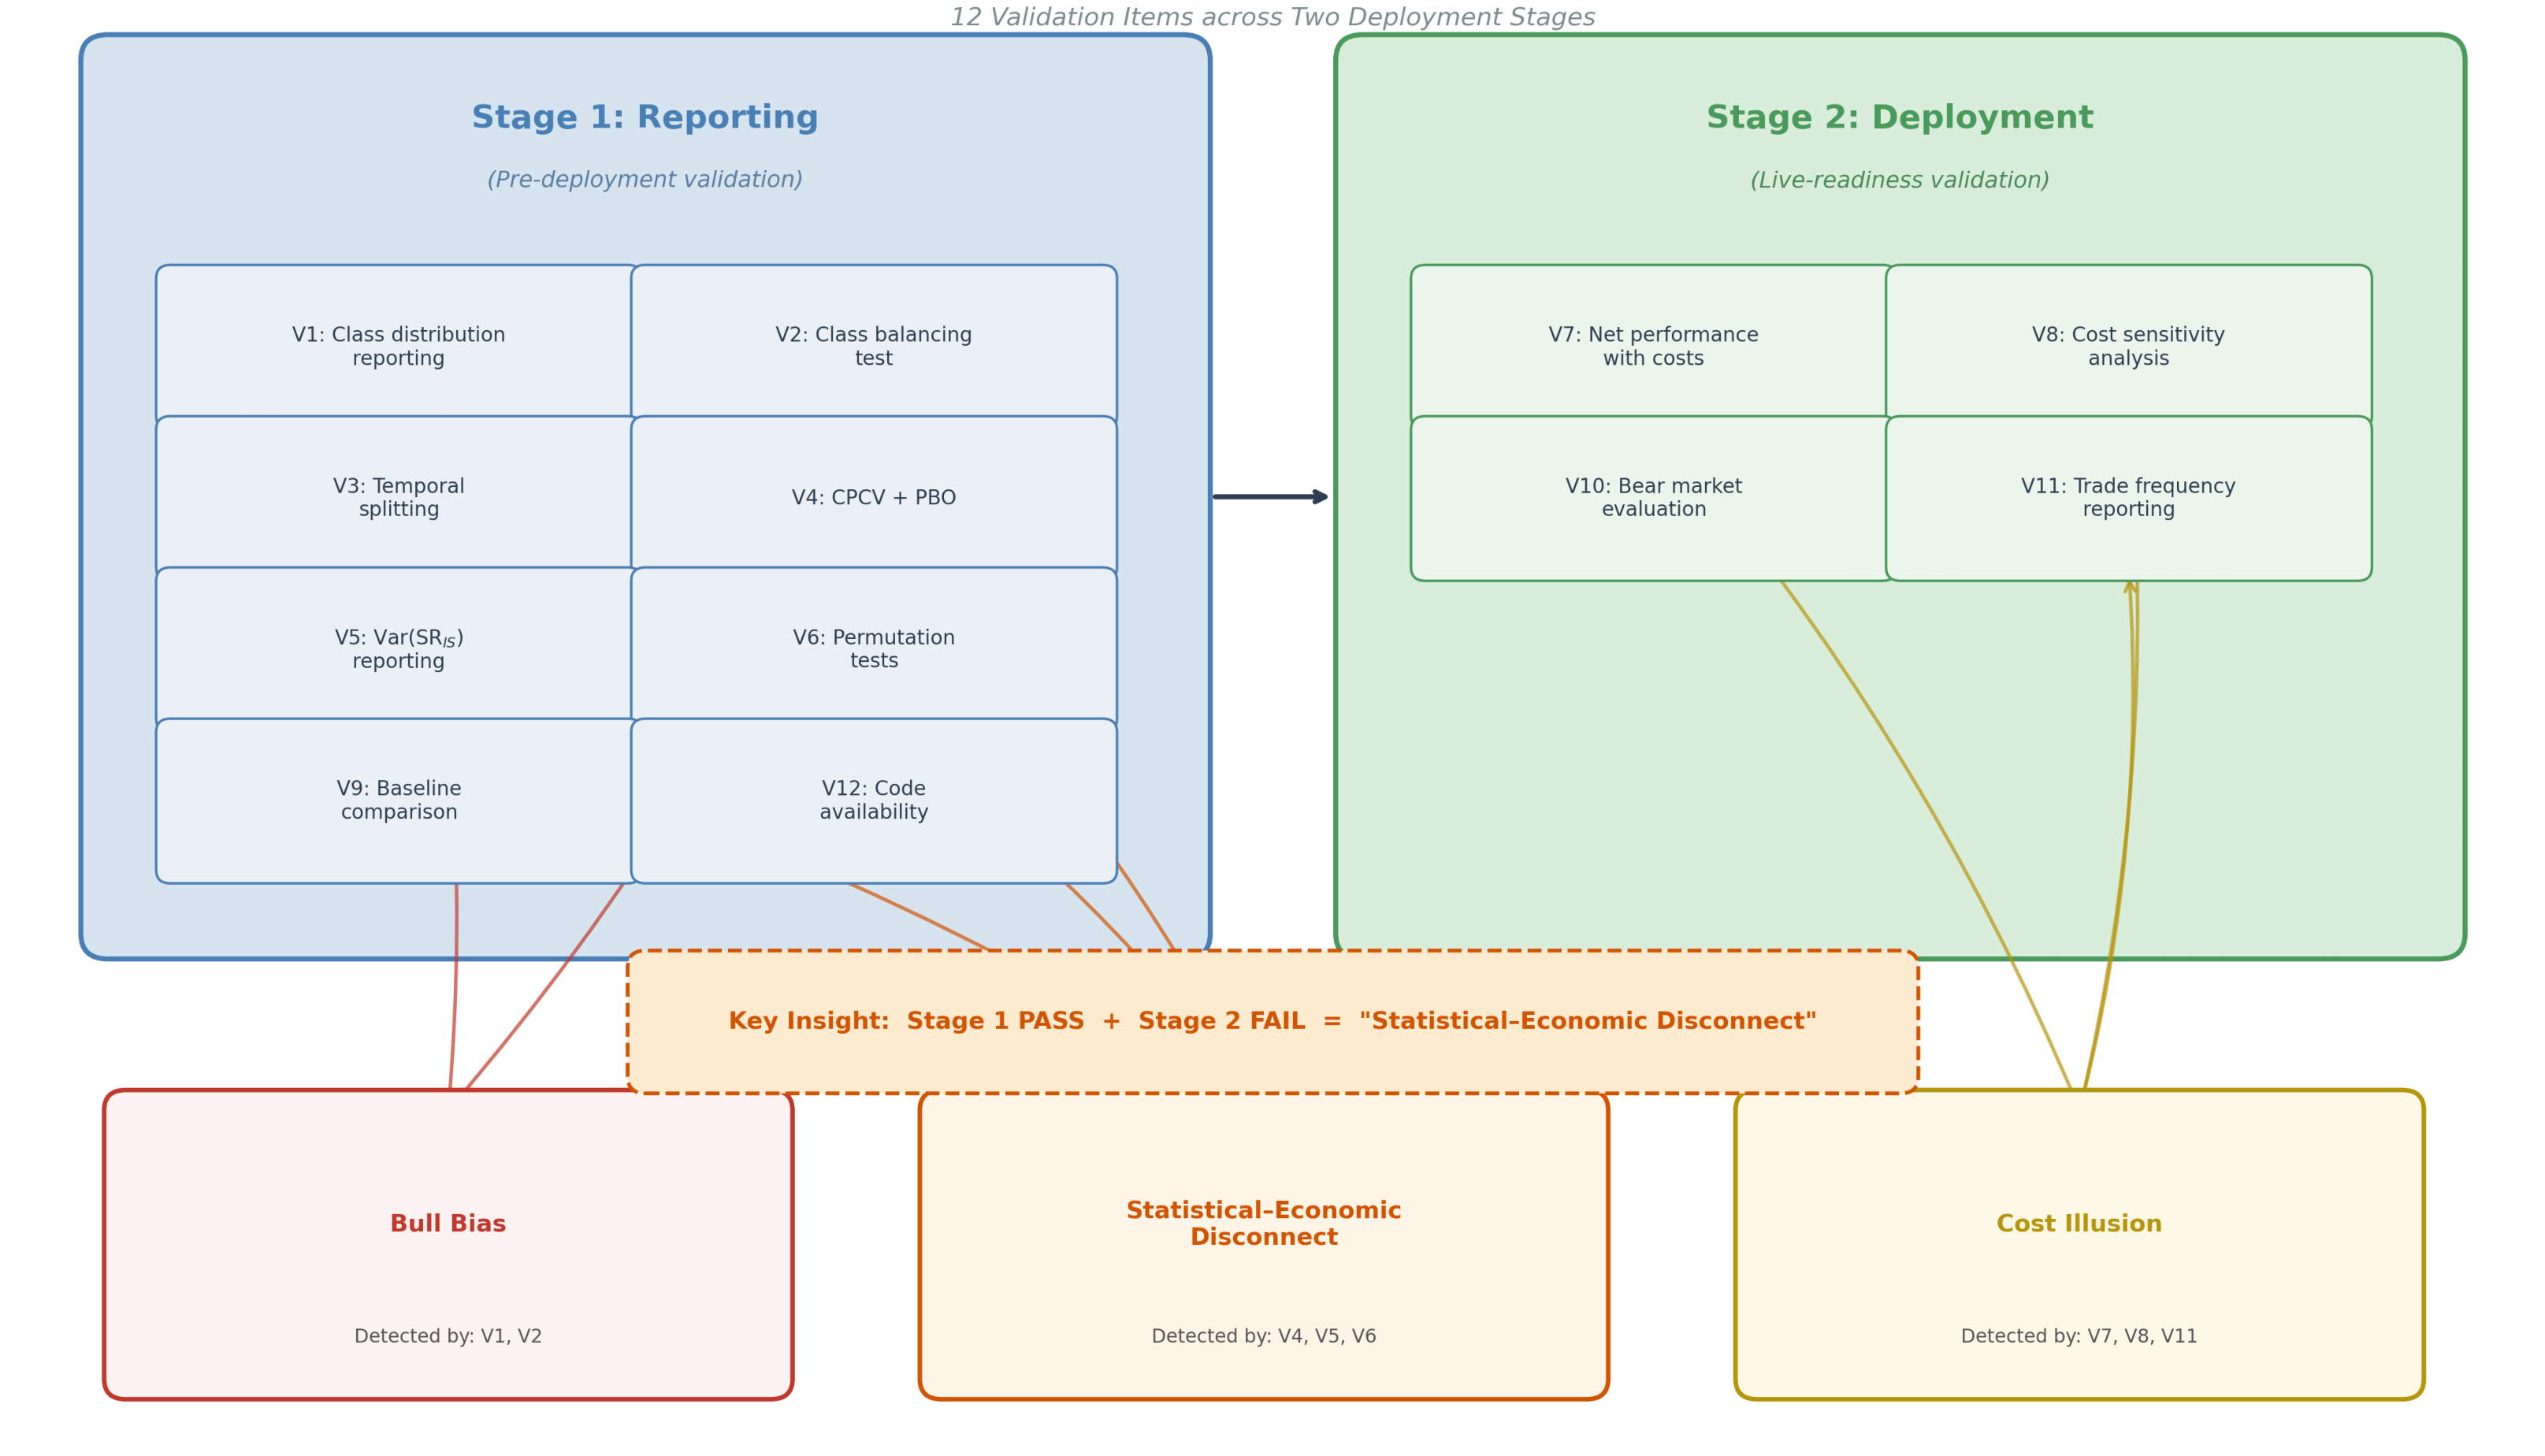
\includegraphics[width=\textwidth]{figures/fig0_valid_overview.png}
\caption{VALID framework overview. Stage~1 (Reporting) items V1--V6, V9, V12 address scientific validity; Stage~2 (Deployment) items V7, V8, V10, V11 address economic viability. Three empirical failure modes are detected by specific item subsets: bull bias (V1, V2), statistical-economic disconnect (V4--V6), and cost illusion (V7, V8, V11). A strategy passing Stage~1 but failing Stage~2 exhibits the statistical-economic disconnect.}
\label{fig:valid_overview}
\end{figure*}

%% ================================================================
\section{Empirical Validation: Three Failure Modes}
\label{sec:empirical}

\subsection{Methodology and Notation}

We deliberately employ standard, well-documented model architectures rather than novel ones, as our objective is to evaluate validation methodology, not to propose new prediction algorithms. This subsection defines the key methods used throughout our experiments.

\subsubsection{Triple Barrier Labeling}
Following \citet{lopezdeprado2018advances}, each observation is assigned a label $y_i \in \{-1, 0, +1\}$ based on the first barrier touched by the price path after event time~$t_i$. Let $p_t$ denote the price at time~$t$. Three barriers are defined:
\begin{align}
\text{Upper:} \quad & p_{t_i + \tau} \geq p_{t_i}(1 + \theta_u) \label{eq:tb_upper} \\
\text{Lower:} \quad & p_{t_i + \tau} \leq p_{t_i}(1 - \theta_l) \label{eq:tb_lower} \\
\text{Vertical:} \quad & \tau = T_{\max} \label{eq:tb_vert}
\end{align}
where $\theta_u, \theta_l > 0$ are profit-taking and stop-loss thresholds scaled to local volatility ($\theta_u = 2.0\hat{\sigma}$, $\theta_l = 2.5\hat{\sigma}$ in our daily configuration; Equations~\ref{eq:tb_upper}--\ref{eq:tb_vert}), and $T_{\max}$ is the maximum holding period. Events are sampled via CUSUM filtering on cumulative log-returns with threshold~$h$.

\subsubsection{Combinatorial Purged Cross-Validation (CPCV)}
Given $N$~chronologically ordered groups and a test size of $k$~groups, CPCV generates $\binom{N}{k}$ unique train-test combinations, each respecting temporal ordering with purge and embargo periods to prevent information leakage. In our configuration ($N = 6$, $k = 2$), this yields $\binom{6}{2} = 15$ combinations, producing $\phi = (k/N)\binom{N}{k} = 5$ non-overlapping backtest paths. For each combination~$j$, a model is trained on the $N - k$ training groups and evaluated on the $k$~test groups, producing an out-of-sample Sharpe ratio $\mathrm{SR}_{\mathrm{OOS}}^{(j)}$.

\subsubsection{Probability of Backtest Overfitting (PBO)}
For each CPCV path, the in-sample-best configuration is identified and its out-of-sample rank $\omega^{(j)} \in \{1, \ldots, M\}$ is recorded. The relative rank is normalized as $\bar{\omega}^{(j)} = \omega^{(j)} / (M+1)$ to avoid boundary values. PBO is defined as:
\begin{equation}
\mathrm{PBO} = \frac{1}{\binom{N}{k}} \sum_{j=1}^{\binom{N}{k}} \mathbf{1}\!\left[\mathrm{logit}(\bar{\omega}^{(j)}) \leq 0\right]
\label{eq:pbo}
\end{equation}
where $\mathrm{logit}(x) = \ln(x / (1-x))$. PBO\,$\approx$\,0 indicates that in-sample-best configurations tend to rank in the top half out-of-sample; PBO\,$\approx$\,1 indicates severe overfitting (Equation~\ref{eq:pbo}; \citealt{bailey2017probability}).

\subsubsection{Parameter-Space Variance}
To diagnose flat parameter landscapes (\citeauthor{witzany2021bayesian}, \citeyear{witzany2021bayesian}), we compute the variance of in-sample Sharpe ratios across all tested configurations:
\begin{equation}
\mathrm{Var}(\mathrm{SR}_{\mathrm{IS}}) = \frac{1}{M-1}\sum_{m=1}^{M}\left(\mathrm{SR}_{\mathrm{IS}}^{(m)} - \overline{\mathrm{SR}}_{\mathrm{IS}}\right)^2
\label{eq:varsr}
\end{equation}
Low $\mathrm{Var}(\mathrm{SR}_{\mathrm{IS}})$ relative to a null distribution (Equation~\ref{eq:varsr}) indicates that all configurations perform similarly, rendering PBO\,=\,0 uninformative rather than reassuring.

\subsection{Strategy Universe}

Our 340 strategy variants are constructed as shown in Table~\ref{tab:universe}:

\begin{table}[htbp]
\centering
\caption{Composition of the 340-variant strategy universe.}
\label{tab:universe}
\small
\resizebox{\columnwidth}{!}{%
\begin{tabular}{clr}
\toprule
Component & Description & Count \\
\midrule
(a) & SHAP-derived rule combinations (applied to momentum benchmark) & 64 \\
(b) & Order flow features (individual + multi-asset) & 55 \\
(c) & External/on-chain/macro feature sets & 45 \\
(d) & ML pipeline: 3 assets $\times$ 4 TF $\times$ 3 tree families & 36 \\
(e) & Triple Barrier parameter sensitivity & 36 \\
(f) & Cross-section momentum configurations & 24 \\
(g) & Cost sensitivity \& traditional baselines & 24 \\
(h) & Deep learning: 3 assets $\times$ 2 TF $\times$ 5 arch.\ (Transformer, LSTM, TCN, MLP$\times$2) & 30 \\
(i) & VALID ablation configurations & 12 \\
(j) & Volatility prediction overlays & 8 \\
(k) & Bull bias analysis (tree + DL) & 6 \\
\midrule
& \textbf{Total unique configurations} & \textbf{340} \\
\bottomrule
\end{tabular}
}
\end{table}

Component~(a) uses SHAP feature attributions \citep{lundberg2017unified} to derive interpretable trading rules from gradient-boosted models. Components (a)--(k) span three cryptocurrency assets (BTC, ETH, SOL), four timeframes (15-minute to daily), and eight model families (CatBoost, LightGBM, Random Forest, Transformer, bidirectional LSTM, TCN, MLP 2-layer, MLP 3-layer). Bull bias analysis (component~k) additionally includes unidirectional LSTM and SimpleRNN. Each was evaluated with 18~bp round-trip costs. All 340 variants were executed through the full ML pipeline; no synthetic or simulated results are included.

\subsection{Failure Mode 1: Bull Bias}

\subsubsection{Experimental Setup}
We train gradient-boosted tree models (CatBoost \citep{prokhorenkova2018catboost}, LightGBM \citep{ke2017lightgbm}, Random Forest) and deep learning models (2-layer LSTM, SimpleRNN) on hourly OHLCV data for BTC, ETH, and SOL with Triple Barrier labeling and CUSUM filtering \citep{lopezdeprado2018advances}. All tree-based methods follow the gradient boosting framework of \citet{friedman2001greedy}, with CatBoost's ordered boosting \citep{dorogush2018catboost} and XGBoost's regularized objective \citep{chen2016xgboost} representing the two dominant implementations in recent crypto ML studies.

\subsubsection{Results}
Table~\ref{tab:bullbias} presents the results.

\begin{table}[htbp]
\centering
\caption{Bull bias across assets and model families.}
\label{tab:bullbias}
\resizebox{\columnwidth}{!}{%
\begin{tabular}{lrrrrr}
\toprule
Asset (Model) & Unbal.\ Long\% & Bal.\ Long\% & AUC (u) & AUC (b) & Net SR \\
\midrule
BTC (CatBoost) & 97.2\% & 42.3\% & 0.502 & 0.501 & $-$0.877 \\
BTC (LSTM) & 57.7\% & 52.3\% & 0.518 & 0.519 & $-$1.149 \\
BTC (SimpleRNN) & 63.3\% & --- & --- & 0.520 & --- \\
ETH (CatBoost) & 90.5\% & 45.2\% & 0.501 & 0.493 & $-$1.283 \\
SOL (CatBoost) & 97.0\% & 32.2\% & 0.533 & 0.511 & $-$0.206 \\
\bottomrule
\end{tabular}
}
\end{table}

Tree-based models exhibit extreme long bias (90--97\%) while deep learning shows moderate-to-strong bias (58--86\% across seven architectures including Transformer, bidirectional LSTM, and TCN). AUC is indistinguishable from random (0.50--0.52) across all model families. Bull bias extends the observation of \citet{jaquart2021short} to a systematic, multi-asset, multi-model phenomenon (see Figure~\ref{fig:bullbias}).

\begin{figure*}[htbp]
\centering
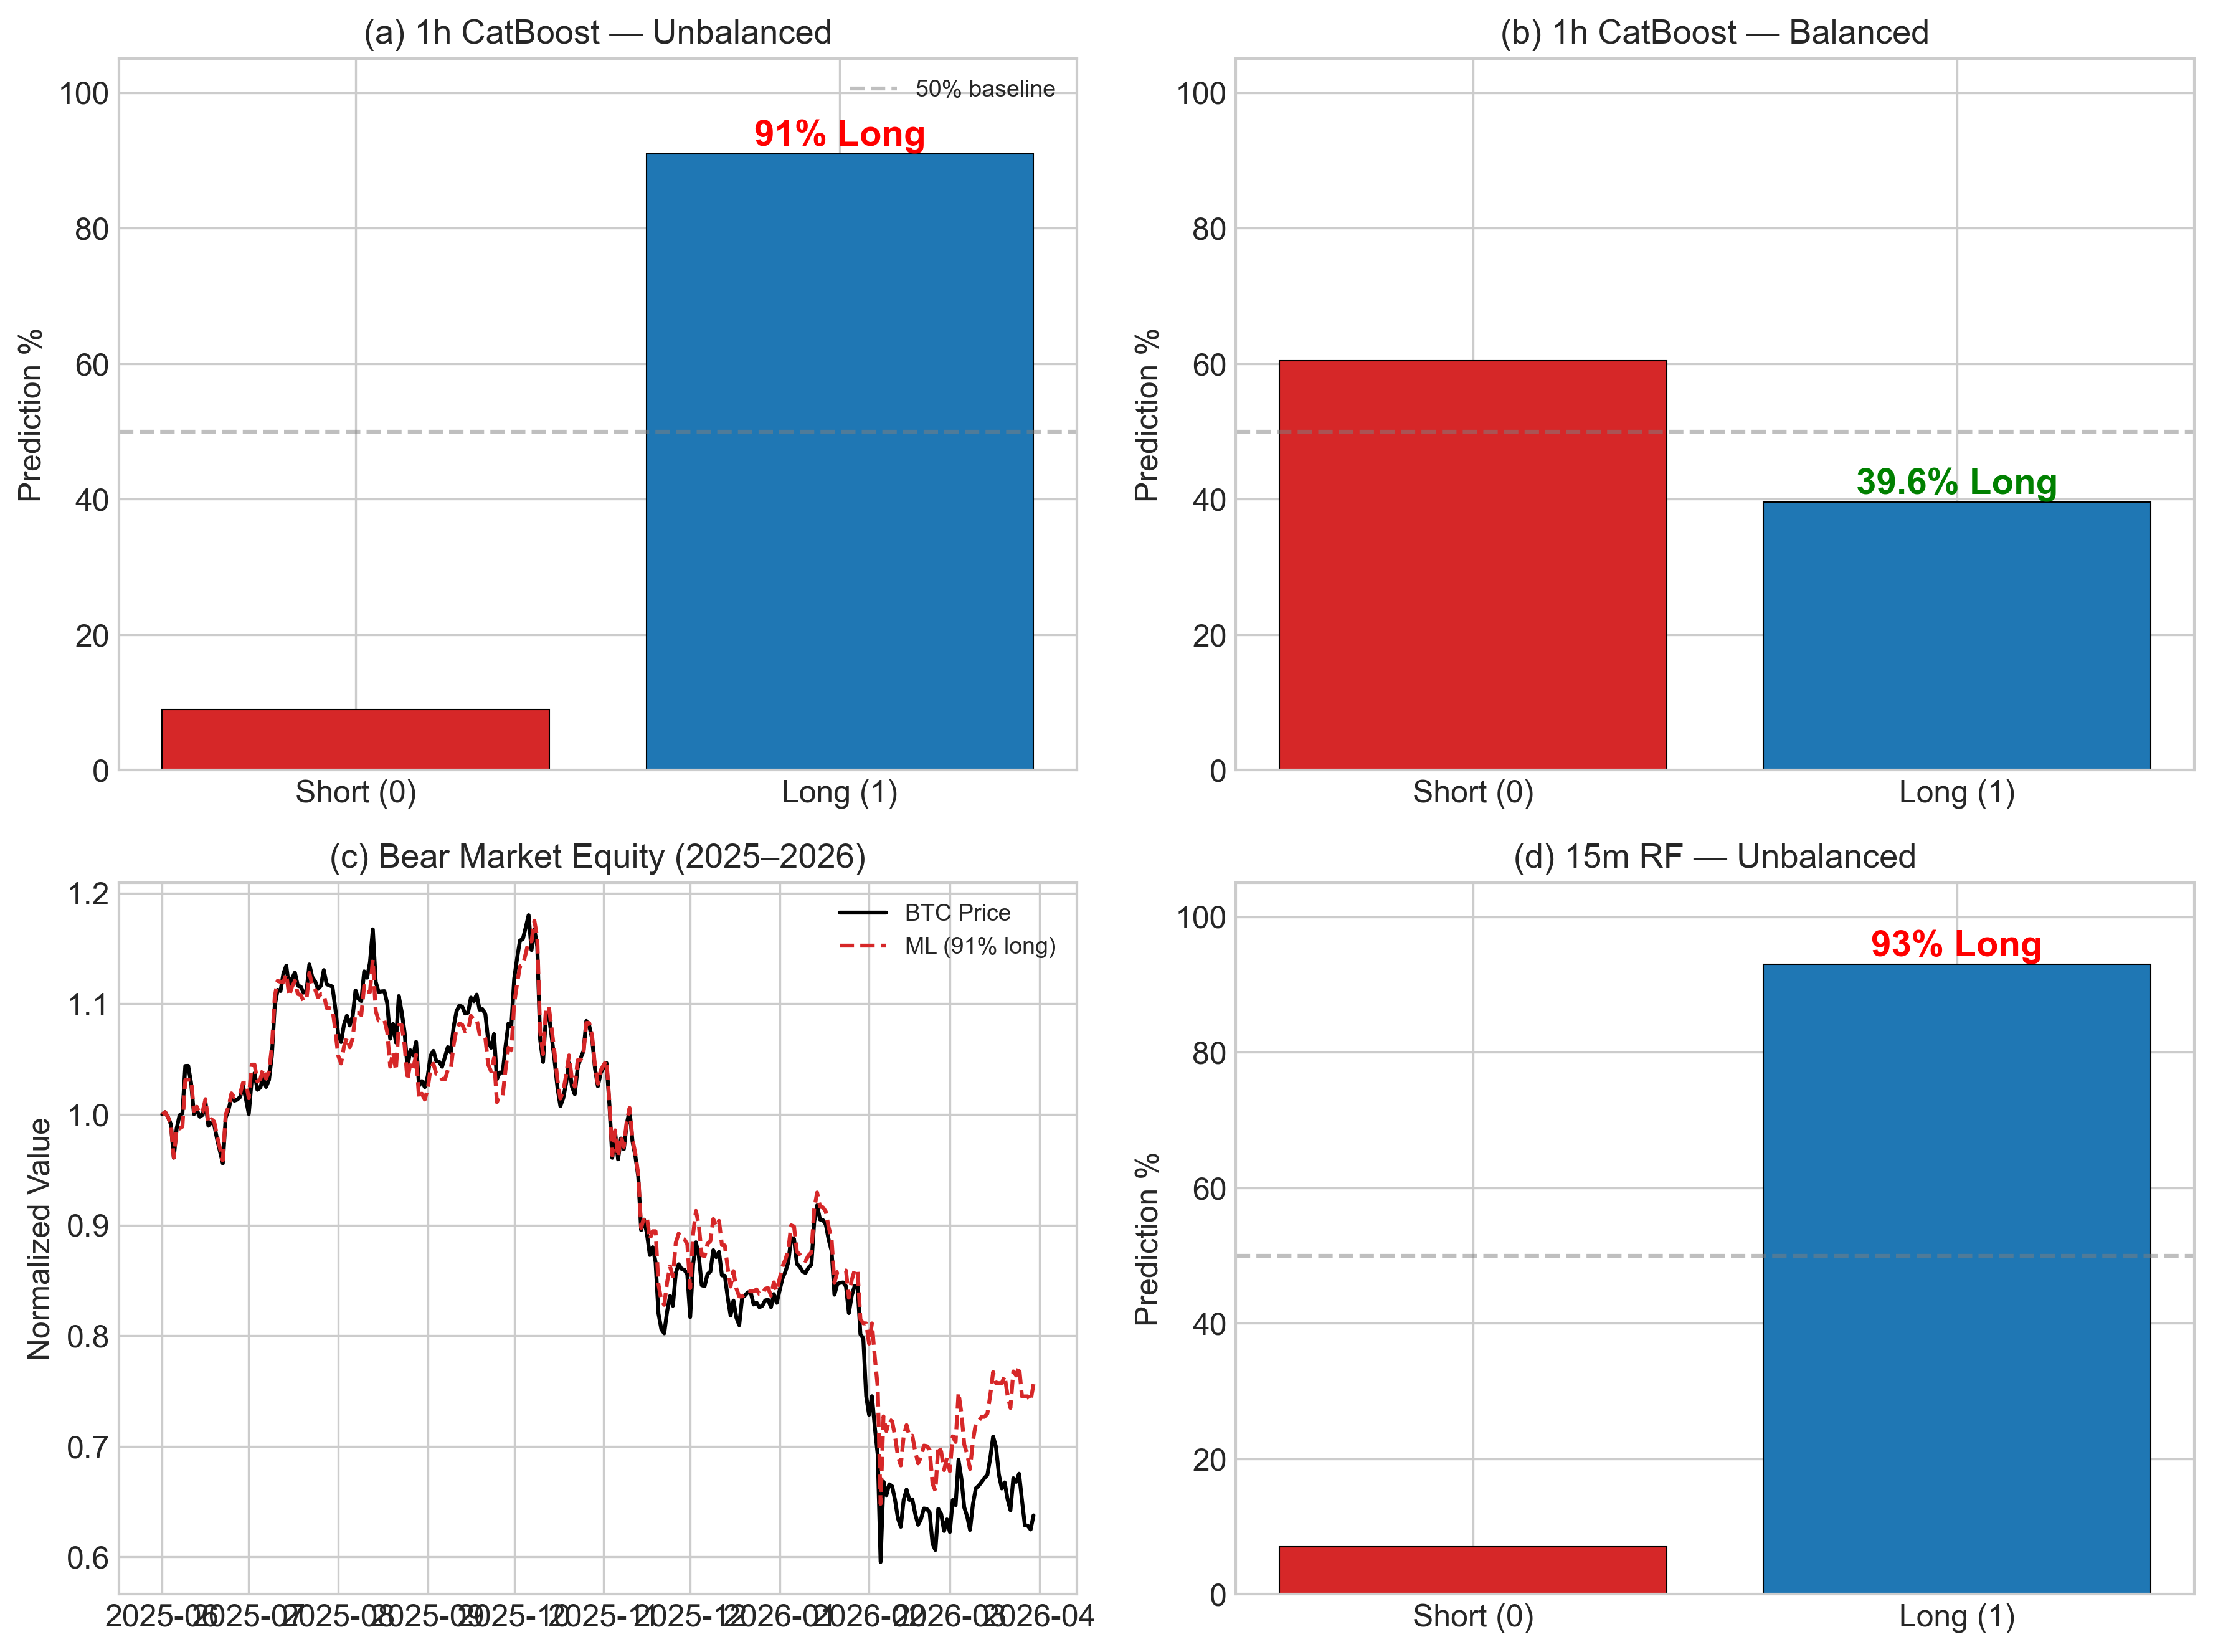
\includegraphics[width=\textwidth]{figures/fig1_bull_bias.png}
\caption{Bull bias in cryptocurrency ML models. (a)~Unbalanced CatBoost predicts 91\% long. (b)~Balanced CatBoost reduces to 39.6\%. (c)~Equity curves during 2025--2026 bear market. (d)~15m RF shows 93\% long bias.}
\label{fig:bullbias}
\end{figure*}

\subsubsection{Extended Multi-Asset Analysis}
To confirm that bull bias is not an artifact of a single asset, timeframe, or model family, we extend the evaluation to 18 asset-timeframe-model combinations: 3 assets $\times$ 2 timeframes (1-hour, daily) $\times$ 3 model families (CatBoost, LightGBM, Random Forest). Table~\ref{tab:multiasset} summarizes the results.

\begin{table}[htbp]
\centering
\caption{Extended multi-asset bull bias (18 combinations).}
\label{tab:multiasset}
\resizebox{\columnwidth}{!}{%
\begin{tabular}{lrrrr}
\toprule
Asset & Mean Unbal.\ Long\% & Mean Bal.\ Long\% & Mean AUC (bal) & Mean Net SR \\
\midrule
BTC & 85\% & 47\% & 0.484 & $-$0.174 \\
ETH & 83\% & 52\% & 0.563 & $+$0.023 \\
SOL & 80\% & 45\% & 0.542 & $+$0.441 \\
\bottomrule
\end{tabular}
}
\end{table}

All assets exhibit unbalanced long ratios of 80--97\% across all models and timeframes. Critically, class balancing eliminates directional bias but does not improve predictive power: balanced AUC remains indistinguishable from random (0.48--0.56) across all 18 asset-model combinations, and mean net SR is negative for BTC ($-$0.174). All 1-hour models receive PBO\,=\,1.000. The phenomenon is timeframe-invariant and asset-invariant.

\subsection{Failure Mode 2: Statistical-Economic Disconnect}

\subsubsection{The Disconnect}
Our 1-hour CatBoost model (balanced) achieves PBO\,=\,0.000 and permutation $p$\,=\,0.000 (AUC 0.570 vs.\ shuffled 95th percentile 0.516). Yet its net SR is only $+$0.135---economically marginal versus a benchmark SR of 0.917. The $\mathrm{Var}(\mathrm{SR}_{\mathrm{IS}})$ is 0.012, which falls below the null distribution (95th percentile\,=\,0.328; see Section~\ref{sec:witzany}). The IS-OOS Spearman correlation is $-$0.08 ($p$\,=\,0.60). This aligns with \citet{harvey2016cross} and \citet{novymarx2016taxonomy} on statistical-economic gaps (see Figure~\ref{fig:pbo}).

\begin{figure*}[htbp]
\centering
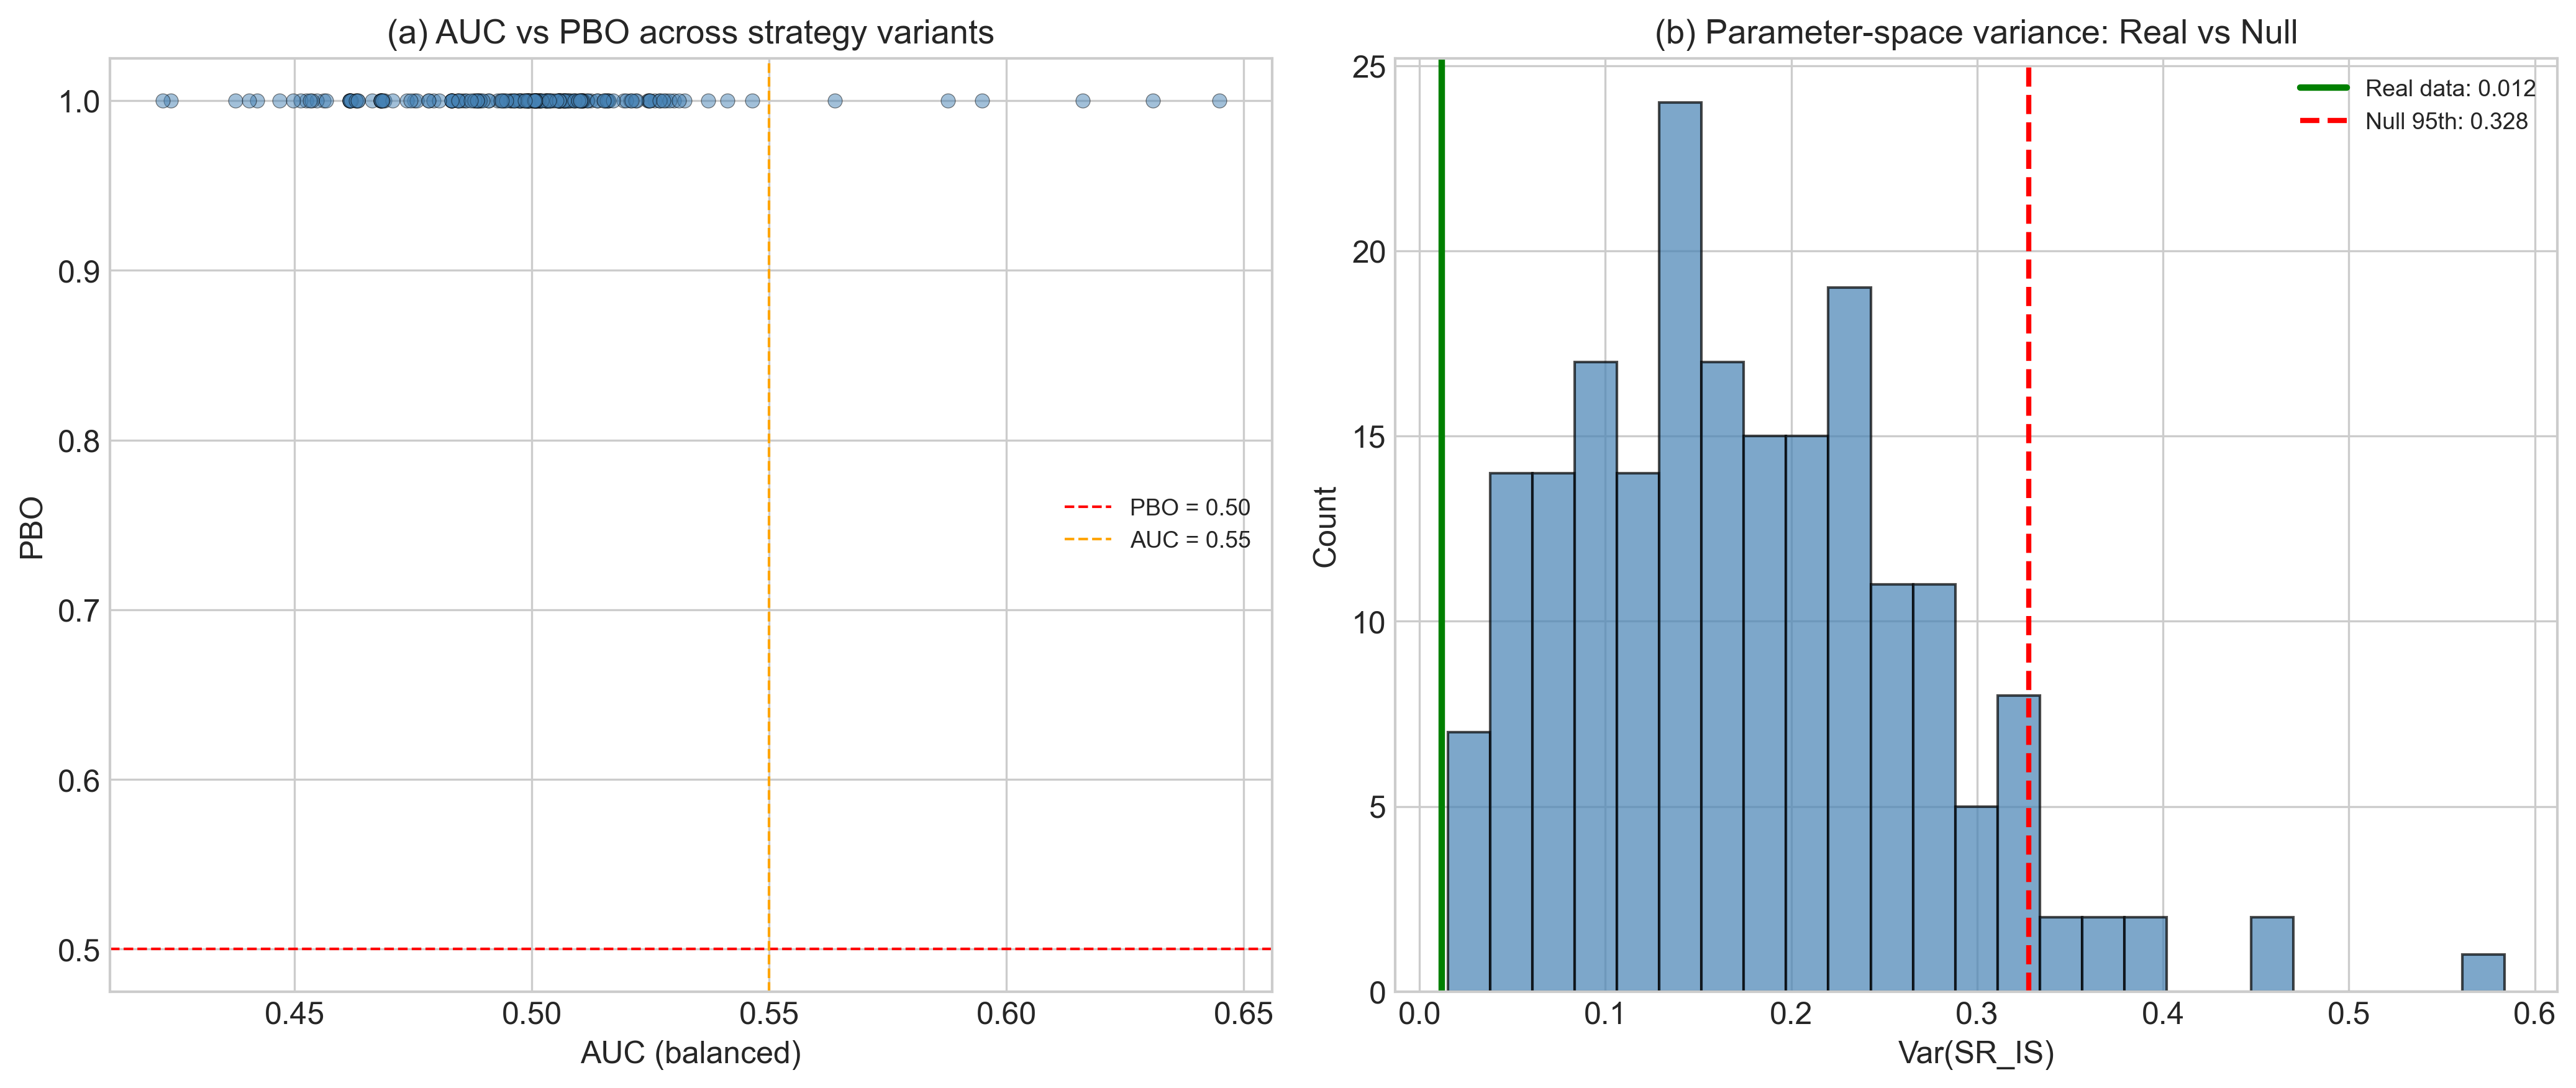
\includegraphics[width=\textwidth]{figures/fig2_pbo_paradox.png}
\caption{The PBO paradox. (a)~AUC vs.\ PBO across strategy variants---nearly all configurations receive PBO close to 1.0, with AUC clustered around 0.50. (b)~Parameter-space variance: the real data's $\mathrm{Var}(\mathrm{SR}_{\mathrm{IS}})$ (green line) falls far below the null distribution (blue histogram), confirming parameter-space flatness.}
\label{fig:pbo}
\end{figure*}

\subsubsection{Parameter-Space Flatness: Empirical Validation of Witzany (2021)}
\label{sec:witzany}

\citet{witzany2021bayesian} demonstrated theoretically that CSCV/PBO exhibits negative bias when strategies have similar returns. \citet{arian2024backtest} compared CPCV variants but did not measure $\mathrm{Var}(\mathrm{SR}_{\mathrm{IS}})$ under null conditions.

We address this gap using 200-iteration Monte Carlo simulation (Section~\ref{sec:montecarlo}). Table~\ref{tab:varsr} compares the real and null distributions:

\begin{table}[htbp]
\centering
\caption{Parameter-space variance: real vs.\ null across four settings.}
\label{tab:varsr}
\begin{tabular}{llll}
\toprule
Setting & Real Data & Null Mean & Null 95th pctl \\
\midrule
BTC 1h & 0.012 & 0.176 & 0.328 \\
ETH 1h & --- & 0.262 & 0.534 \\
SOL 1h & --- & 0.296 & 0.617 \\
BTC daily & --- & 0.176 & 0.328 \\
\bottomrule
\end{tabular}
\end{table}

The real data's parameter-space variance falls dramatically below the null distribution. This confirms Witzany's critique empirically: PBO\,=\,0 in our setting reflects parameter-space flatness rather than genuine signal robustness. We propose that if $\mathrm{Var}(\mathrm{SR}_{\mathrm{IS}})$ falls below the 5th percentile of a null distribution ($\approx$0.02), PBO should be flagged as reflecting parameter-space flatness.

\subsubsection{Monte Carlo Confirmation}

Monte Carlo analysis (Section~\ref{sec:montecarlo}) confirms these findings on synthetic data: AUC-based validation alone produces 27\% false positives, while PBO eliminates all false positives (0\% FPR, upper bound 1.9\%). Full results are reported in Table~\ref{tab:fpr}.\footnote{Permutation test results are based on the first 100 iterations ($n$\,=\,100); all other criteria are evaluated across all 200 iterations.}

\subsection{Failure Mode 3: Cost Illusion}

\subsubsection{Cross-Timeframe Cost Analysis}

Table~\ref{tab:cost} presents cost sensitivity across timeframes.

\begin{table}[htbp]
\centering
\caption{Cost sensitivity: benchmark vs.\ ML Sharpe ratios.}
\label{tab:cost}
\begin{tabular}{lrrr}
\toprule
Cost (RT bp) & Benchmark SR & 1h ML SR & 15m ML SR \\
\midrule
0 & 0.954 & 0.640 & 0.416 \\
18 & 0.917 & 0.530 & 0.186 \\
50 & 0.852 & 0.335 & $-$0.222 \\
\bottomrule
\end{tabular}
\end{table}

ML strategies fail to beat frequency-matched baselines at every cost level, including zero. Even institutional traders with near-zero costs cannot rescue ML alpha (SR 0.640 vs.\ 0.804 for RSI at 0~bp). Cost drag (55--91\%) exacerbates signal weakness but does not cause it. The 15-minute results (all 9 variants with SR\,$<$\,$-$1.3) serve as a robustness check confirming that higher-frequency execution amplifies the failure (see Figure~\ref{fig:cost}).

Our 18~bp fixed round-trip cost is conservative for hourly and daily frequencies (Binance taker fee: 10~bp + estimated slippage of 5--10~bp; \citealt{almeida2024microstructure}). For sub-hourly frequencies, volume-dependent slippage models \citep{almgren2001optimal} would further erode returns, strengthening rather than weakening our conclusions.

\begin{figure}[htbp]
\centering

\includegraphics[width=\columnwidth]{figures/fig3_cost_illusion.png}
\caption{The cost illusion: gross vs.\ net Sharpe ratio by timeframe. Cost drag increases monotonically with trading frequency, consuming 91\% of alpha at 15-minute frequency.}
\label{fig:cost}
\end{figure}

\subsubsection{Comparison with Traditional Baselines}

To ensure fair comparison across different trading frequencies, we group baselines by rebalancing frequency (Table~\ref{tab:baselines}) and compare each ML variant against a frequency-matched alternative.

\begin{table}[htbp]
\centering
\caption{Strategy comparison by frequency band (18~bp round-trip costs).}
\label{tab:baselines}
\resizebox{\columnwidth}{!}{%
\begin{tabular}{llrrrr}
\toprule
Frequency & Strategy & CAGR & MDD & SR (net) & Trades/yr \\
\midrule
\multirow{2}{*}{\textit{Low (monthly)}} & Dual momentum$^\dagger$ & 42.8\% & $-$51.3\% & 0.917 & 9.7 \\
& SMA 200 crossover & 33.1\% & $-$64.6\% & 0.723 & 7.6 \\
\midrule
\multirow{3}{*}{\textit{Medium (daily)}} & RSI(14) $>$ 50 & 38.4\% & $-$54.1\% & 0.804 & 44.0 \\
& MACD crossover & 25.2\% & $-$55.0\% & 0.613 & 26.2 \\
& 1h ML (CatBoost, bal.) & 19.4\% & $-$62.6\% & 0.530 & 30.8 \\
\midrule
\textit{Passive} & Buy \& Hold & 30.6\% & $-$76.6\% & 0.618 & 0.1 \\
\bottomrule
\multicolumn{6}{l}{\footnotesize $^\dagger$Upper-bound reference following \citet{antonacci2014dual}; monthly rebalancing not directly comparable to intraday ML.}
\end{tabular}
}
\end{table}

Within the frequency-matched comparison, the best ML strategy (SR\,=\,0.530, 31 trades/year) underperforms both RSI (SR\,=\,0.804, 44 trades/year) and MACD (SR\,=\,0.613, 26 trades/year) despite comparable trading frequency. The dual momentum benchmark serves as an upper-bound reference; its superior SR reflects lower turnover (9.7 trades/year) rather than superior signal quality. Cross-section momentum strategies (24 configurations across 7 lookback periods and 3 portfolio sizes) similarly fail, with only 4 of 24 achieving SR\,$>$\,0 (see Figures~\ref{fig:complexity}, \ref{fig:regime}, and~\ref{fig:distribution}).

\begin{figure}[htbp]
\centering

\includegraphics[width=\columnwidth]{figures/fig4_complexity.png}
\caption{Complexity vs.\ performance: adding rules monotonically degrades Sharpe ratio (slope $= -0.065$ per rule).}
\label{fig:complexity}
\end{figure}

\begin{figure}[htbp]
\centering

\includegraphics[width=\columnwidth]{figures/fig5_regime.png}
\caption{Regime-conditional performance. The momentum benchmark earns SR\,=\,1.40 in stressed regimes vs.\ 0.79 for buy-and-hold---alpha concentrates during market stress.}
\label{fig:regime}
\end{figure}

\begin{figure}[htbp]
\centering

\includegraphics[width=\columnwidth]{figures/fig6_482_distribution.png}
\caption{Distribution of net Sharpe ratios across 340 strategy variants. The benchmark (green line) exceeds the vast majority of ML variants. 52\% of variants produce negative SR.}
\label{fig:distribution}
\end{figure}

\subsection{Ablation Analysis: Which VALID Items Matter Most?}

Table~\ref{tab:ablation} presents the ablation results.

\begin{table}[htbp]
\centering
\caption{Ablation: false positive rates by VALID item removal.}
\label{tab:ablation}
\begin{tabular}{llrl}
\toprule
Configuration & Items Removed & FPR & 95\% Wilson CI \\
\midrule
Full VALID & None & 0.0\% & [0.0\%, 1.9\%] \\
No CPCV/PBO & $-$V4 & 27.0\% & [21.3\%, 33.5\%] \\
No balancing & $-$V2 & 0.0\% & [0.0\%, 5.8\%] \\
No cost adj. & $-$V7 & 0.0\% & [0.0\%, 1.9\%] \\
No permutation & $-$V6 & 0.0\% & [0.0\%, 1.9\%] \\
\bottomrule
\end{tabular}
\end{table}

V4 (CPCV/PBO) is the single most important item. Its removal causes FPR to increase from 0\% to 27\%.

%% ================================================================
\section{Monte Carlo False Positive Analysis}
\label{sec:montecarlo}

\subsection{Motivation and Definitions}

The empirical results in Section~\ref{sec:empirical} demonstrate failure modes on real data, but a natural question arises: how often would standard validation tools produce false positives on data with \textit{no embedded signal}? We address this through Monte Carlo simulation.

We define a \textbf{false positive} as a null (signal-free) dataset on which a given validation criterion incorrectly indicates the presence of a tradable signal. Specifically, for each criterion $C$ and null dataset $i$, let $\mathrm{FP}_i = \mathbf{1}[C_i \text{ passes}]$. The false positive rate is:
\begin{equation}
\mathrm{FPR}(C) = \frac{1}{n}\sum_{i=1}^{n} \mathrm{FP}_i
\label{eq:fpr}
\end{equation}
with 95\% Wilson confidence intervals \citep{wilson1927probable}. We evaluate five criteria: AUC\,$>$\,0.55, permutation test $p$\,$<$\,0.05, PBO\,$<$\,0.20, net SR\,$>$\,0, and the conjunction of all VALID items.

\subsection{Synthetic Data Generation}
We generate $n$\,=\,200 synthetic BTC price series by bootstrapping \citep{efron1993bootstrap} daily log-returns (2017--2026, 3{,}132 observations per series). The bootstrap preserves the marginal distribution of returns (mean, variance, skewness, kurtosis) while destroying temporal dependence, ensuring that any predictive signal detected by the ML pipeline is spurious by construction. We use simple i.i.d.\ resampling rather than block or stationary bootstrap \citep{politis1994stationary}, as our goal is to eliminate all temporal structure. The choice of $n$\,=\,200 yields Wilson CI half-widths of $\pm$6\% at FPR\,=\,27\%, providing sufficient precision to distinguish informative from uninformative validation criteria.

\subsection{Pipeline Application}
Each synthetic series passes through the identical pipeline used for real data: (a)~compute 17 price-derived technical features (returns, volatility, momentum indicators); (b)~generate Triple Barrier labels with CUSUM filtering; (c)~train CatBoost with class-balanced sample weights; (d)~evaluate via CPCV ($N$\,=\,6, $k$\,=\,2, yielding 15 train-test combinations); (e)~record AUC, PBO, $\mathrm{Var}(\mathrm{SR}_{\mathrm{IS}})$, permutation $p$-value, and net SR (18~bp round-trip cost). The pipeline is deterministic given the input data; no hyperparameter tuning is performed within the Monte Carlo loop.

\subsection{Results}
Mean AUC across 200 null iterations is 0.506\,$\pm$\,0.070, confirming that the pipeline produces near-chance classification on signal-free data. However, individual criteria show dramatically different false positive rates (Table~\ref{tab:fpr}; Equation~\ref{eq:fpr}). The 27\% AUC-based FPR, combined with the audit finding that no empirical paper in our sample uses CPCV, suggests a substantial fraction of published positive results may reflect statistical artifacts. Critically, PBO\,$<$\,0.20 alone achieves 0\% FPR [0\%, 1.9\%], confirming its value as the primary overfitting diagnostic and justifying its central role in VALID (Item V4).

To confirm generalizability, we replicate the Monte Carlo analysis across three additional settings: ETH 1h, SOL 1h, and BTC daily (Table~\ref{tab:fpr}). AUC-based FPR ranges from 26.5\% to 30.0\% across all four settings, while PBO-based FPR remains 0.0\% in every case. The consistency of these results across assets (BTC, ETH, SOL) and timeframes (hourly, daily) confirms that the findings are asset-invariant and timeframe-invariant: standard validation criteria produce false positives at similar rates regardless of the underlying data, and CPCV with PBO eliminates them universally.

\begin{table}[htbp]
\centering
\caption{False positive rates on null data ($n$\,=\,200 per setting). BTC 1h is the primary setting; three additional settings confirm generalizability.}
\label{tab:fpr}
\small
\begin{tabular}{lrrrr}
\toprule
Criterion & BTC 1h & ETH 1h & SOL 1h & BTC daily \\
\midrule
AUC $>$ 0.55 alone & 27.0\% & 30.0\% & 26.5\% & 27.0\% \\
Permutation passed & 22.0\% & 19.0\% & 18.0\% & 20.0\% \\
PBO $<$ 0.20 alone & 0.0\% & 0.0\% & 0.0\% & 0.0\% \\
Net SR $>$ 0 alone & 49.5\% & 52.0\% & 52.5\% & 49.5\% \\
Full VALID & 0.0\% & 0.0\% & 0.0\% & 0.0\% \\
\bottomrule
\end{tabular}
\end{table}

%% ================================================================
\section{Discussion}
\label{sec:discussion}

\subsection{Implications for the Field}

Our findings have four implications. First, the crypto ML literature likely contains a substantial false positive rate---across our 340 strategy variants, 52\% produce negative net Sharpe ratios after realistic transaction costs, and only 4.4\% exceed the simple momentum benchmark (SR\,=\,0.917). Second, our Monte Carlo analysis provides empirical validation of \citeauthor{witzany2021bayesian}'s (\citeyear{witzany2021bayesian}) theoretical critique of PBO---to our knowledge, the first such test against a null distribution. Third, the statistical-economic disconnect is not a failure of existing tools but a gap in how they are applied. Fourth, the VALID framework addresses a genuine gap---no existing reporting standard covers financial-ML-specific pitfalls.

\subsubsection{Adoption Barriers}
The VALID framework imposes computational and reporting overhead that may deter adoption, particularly for research groups without access to high-performance computing. CPCV with $\binom{6}{2} = 15$ combinations requires 15 full model training runs per configuration, and Monte Carlo analysis with 200 iterations multiplies this further. We view this cost as appropriate: if a validation procedure is too expensive to run, the strategy search itself may be too expansive to be trustworthy. Nonetheless, we acknowledge that pragmatic compromises---such as reducing $N$ or using fewer Monte Carlo iterations---may be necessary for large-scale strategy searches, provided authors disclose the reduced scope.

\subsubsection{Relationship to Publication Incentives}
The failure modes documented in this paper are not primarily technical failures but incentive failures. Journals and conferences reward novelty and positive results; negative results---such as our finding that 52\% of strategy variants produce negative net returns---are difficult to publish. The VALID framework cannot resolve this structural problem, but by mandating disclosure of class distributions, cost-adjusted performance, and baseline comparisons, it raises the evidentiary bar for claiming positive results. We note that analogous reporting standards in clinical research \citep[CONSORT;][]{moher2010consort,collins2015tripod} have measurably improved methodological quality over time, though compliance remains imperfect.

\subsubsection{Generalizability Beyond Cryptocurrency}
While our empirical validation focuses on cryptocurrency markets, the three failure modes---directional prediction bias, statistical-economic disconnect, and cost illusion---are not crypto-specific. Bull bias arises whenever training labels are imbalanced, which occurs in any trending asset class. The statistical-economic disconnect exists wherever statistical validation tools lack economic grounding. Cost illusion affects any strategy with non-trivial turnover. We expect VALID to be applicable, with minor parameter adjustments, to equity factor models, FX strategies, and commodity trading algorithms.

\subsection{Limitations}

Our analysis is subject to several limitations. First, we evaluate three cryptocurrency assets (BTC, ETH, SOL); extending to a broader universe including equities, foreign exchange, or fixed income would strengthen generalizability claims. Second, the VALID framework has not been validated through a formal expert consensus process such as a Delphi study, which is standard for clinical reporting guidelines (TRIPOD, CONSORT). Third, the momentum benchmark operates at monthly rebalancing frequency while ML strategies trade hourly to daily; although we provide frequency-matched comparisons using RSI and MACD (Table~\ref{tab:baselines}), the cross-frequency comparison warrants caution. Fourth, our deep learning evaluation covers five architectures but omits Temporal Fusion Transformers \citep{lim2021temporal} and graph neural networks, which may exploit cross-asset dependencies not captured here. Fifth, the literature audit was conducted by a single coder without independent inter-rater reliability assessment, introducing potential coding bias. Sixth, the audit covers only published and indexed papers, creating survivorship bias---unpublished negative results are absent by construction. Seventh, our 18~bp fixed cost model, while conservative for hourly and daily frequencies, does not capture the volume-dependent slippage dynamics relevant to sub-minute execution.

\subsection{Future Work}

Three extensions merit investigation. First, applying VALID retroactively to highly cited papers would quantify how many published results survive rigorous validation. Second, extending the framework to reinforcement learning strategies---which face additional challenges in reward shaping and environment non-stationarity---would broaden applicability. Third, developing an automated VALID compliance tool, analogous to existing TRIPOD adherence checkers, would lower adoption barriers.

%% ================================================================
\section{Conclusion}
\label{sec:conclusion}

We propose VALID, the first domain-specific validation framework for financial ML. Through a systematic audit of 80 papers, 340 strategy variants across three assets and four timeframes, 800-iteration Monte Carlo analysis across four asset-timeframe settings, and ablation testing, we demonstrate three systematic failure modes: bull bias (90--97\% for tree models, 58--86\% across seven deep learning architectures), statistical-economic disconnect, and cost illusion (55--91\%), with 52\% of all tested variants producing negative returns after costs and only 4.4\% exceeding a simple momentum benchmark. We provide the first empirical confirmation of \citeauthor{witzany2021bayesian}'s (\citeyear{witzany2021bayesian}) PBO critique, with $\mathrm{Var}(\mathrm{SR}_{\mathrm{IS}})$\,=\,0.012 falling far below the null distribution (95th percentile\,=\,0.328). The VALID framework's 12 items would establish minimum reporting standards for a field that currently lacks them.

In a field where positive results are rewarded and negative results are invisible, the most important validation is the discipline to accept that a statistically detectable signal is not the same as a tradable edge.

%% ================================================================
\section*{CRediT Authorship Contribution Statement}

\textbf{Jaewook Kim}: Conceptualization, Methodology, Software, Validation, Formal analysis, Investigation, Data curation, Writing -- original draft, Writing -- review \& editing, Visualization.

%% ================================================================
\section*{Declaration of Competing Interest}

The author declares that there is no known competing financial interest or personal relationship that could have appeared to influence the work reported in this paper.

%% ================================================================
\section*{Acknowledgments}

The author thanks the anonymous reviewers for their constructive feedback.

%% ================================================================
\section*{Funding}

This research did not receive any specific grant from funding agencies in the public, commercial, or not-for-profit sectors.

%% ================================================================
\section*{Data Availability}

Bitcoin, Ethereum, and Solana OHLCV data were obtained from Binance and Bybit public APIs via the CCXT library. Macro indicators were obtained from Yahoo Finance. The literature audit coding sheet, Monte Carlo results, and 340-variant data are provided in supplementary materials. Source code is available at \url{https://github.com/orcajae/valid-framework}.

%% ================================================================
\section*{Appendix A: VALID Self-Assessment}

To demonstrate the framework's application, Table~\ref{tab:selfassess} applies VALID to the present study. This self-assessment serves as a worked example for future adopters.

\begin{table}[htbp]
\centering
\caption{VALID self-assessment applied to this study.}
\label{tab:selfassess}
\footnotesize
\begin{tabular}{clcl}
\toprule
\# & Item & Status & Evidence \\
\midrule
V1 & Class distribution reported & \checkmark & Table~\ref{tab:bullbias}: 90--97\% long \\
V2 & Balanced/unbalanced comparison & \checkmark & Tables~\ref{tab:bullbias},~\ref{tab:multiasset} \\
V3 & Temporal splitting only & \checkmark & CPCV with purge \& embargo \\
V4 & CPCV with PBO & \checkmark & $N$\,=\,6, $k$\,=\,2, 15 combinations \\
V5 & $\mathrm{Var}(\mathrm{SR}_{\mathrm{IS}})$ reported & \checkmark & Table~\ref{tab:varsr}: 0.012 vs.\ null 0.328 \\
V6 & Permutation tests & $\triangle$ & $p$\,=\,0.000; 100 iterations (not 200) \\
V7 & Net performance with costs & \checkmark & 18~bp RT; Table~\ref{tab:cost} \\
V8 & Cost sensitivity analysis & \checkmark & 0, 18, 50~bp in Table~\ref{tab:cost} \\
V9 & Simple baselines & \checkmark & RSI, MACD, SMA in Table~\ref{tab:baselines} \\
V10 & Bear market evaluation & $\triangle$ & Figure~\ref{fig:regime}: two regimes only \\
V11 & Trade frequency reported & \checkmark & Trades/yr in Table~\ref{tab:baselines} \\
V12 & Code available & \checkmark & GitHub repository linked \\
\midrule
& \textbf{Total} & \textbf{10/12} & \textbf{2 partial} \\
\bottomrule
\end{tabular}
\end{table}

\section*{Appendix B: Supplementary Materials}

Supplementary materials include: (A)~complete 340-variant performance results; (B)~VALID framework implementation code; (C)~literature audit coding sheet and raw data for all 80 papers; (D)~Monte Carlo simulation details and per-iteration results (200 iterations).

\bibliography{references}
\bibliographystyle{elsarticle-harv}

\end{document}